% $Id: template.tex 11 2007-04-03 22:25:53Z jpeltier $

\documentclass{vgtc}                          % final (conference style)
%\documentclass[review]{vgtc}                 % review
%\documentclass[widereview]{vgtc}             % wide-spaced review
%\documentclass[preprint]{vgtc}               % preprint
%\documentclass[electronic]{vgtc}             % electronic version

%% Uncomment one of the lines above depending on where your paper is
%% in the conference process. ``review'' and ``wide review'' are for review
%% submission, ``preprint'' is for pre-publication, and the final version
%% doesn't use a specific qualifier. Further, ``electronic'' includes
%% hyperreferences for more convenient online viewing.

%% Please use one of the ``review'' options in combination with the
%% assigned online id (see below) ONLY if your paper uses a double blind
%% review process. Some conferences, like IEEE Vis and InfoVis, have NOT
%% in the past.

%% Figures should be in CMYK or Grey scale format, otherwise, color 
%% shifting may occur during the printing process.

%% These three lines bring in essential packages: ``mathptmx'' for Type 1 
%% type faces, ``graphics'' for inclusion of E'S figures. and ``times''
%% for proper handling of the times font family.

\usepackage{mathptmx}
\usepackage{graphicx}
\usepackage{times}
\usepackage{color}

%% We encourage the use of mathptmx for consistent usage of times font
%% throughout the proceedings. However, if you encounter conflicts
%% with other math-related packages, you may want to disable it.

%% If you are submitting a paper to a conference for review with a double
%% blind reviewing process, please replace the value ``0'' below with your
%% Online-ID. Otherwise, you may safely leave it at ``0''.
\onlineid{0}

%% declare the category of your paper, only shown in review mode
\vgtccategory{Research}

%% allow for this line if you want the electronic option to work properly
\vgtcinsertpkg

%% In preprint mode you may define your own headline.
%\preprinttext{To appear in an IEEE VGTC sponsored conference.}

%% Paper title.

\title{Visualizing the dynamics of enzyme annotations in UniProt/SwissProt}

%% This is how authors are specified in the conference style

%% Author and Affiliation (single author).
%%\author{Roy G. Biv\thanks{e-mail: roy.g.biv@aol.com}}
%%\affiliation{\scriptsize Allied Widgets Research}

%% Author and Affiliation (multiple authors with single affiliations).
%%\author{Roy G. Biv\thanks{e-mail: roy.g.biv@aol.com} %
%%\and Ed Grimley\thanks{e-mail:ed.grimley@aol.com} %
%%\and Martha Stewart\thanks{e-mail:martha.stewart@marthastewart.com}}
%%\affiliation{\scriptsize Martha Stewart Enterprises \\ Microsoft Research}

%% Author and Affiliation (multiple authors with multiple affiliations)
\author{Sabrina A. Silveira\thanks{e-mail: sabrina@dcc.ufmg.br}\\ %
        \scriptsize Universidade Federal de Minas Gerais %
\and Artur O. Rodrigues\thanks{e-mail: artur@dcc.ufmg.br} \\ %
        \scriptsize Universidade Federal de Minas Gerais\\ %
\and Raquel C. de Melo-Minardi\thanks{e-mail: raquelcm@dcc.ufmg.br}\\ %
     \scriptsize Universidade Federal de Minas Gerais\\ %
\\
\and Carlos Henrique da Silveira\thanks{e-mail: carlos.silveira@unifei.edu.br}\\ %
     \scriptsize Universidade Federal de Itajub\'a %
\and Wagner Meira Jr.\thanks{e-mail: meira@dcc.ufmg.br}\\ %
     \scriptsize Universidade Federal de Minas Gerais
}

%% A teaser figure can be included as follows, but is not recommended since
%% the space is now taken up by a full width abstract.
\teaser{\\
  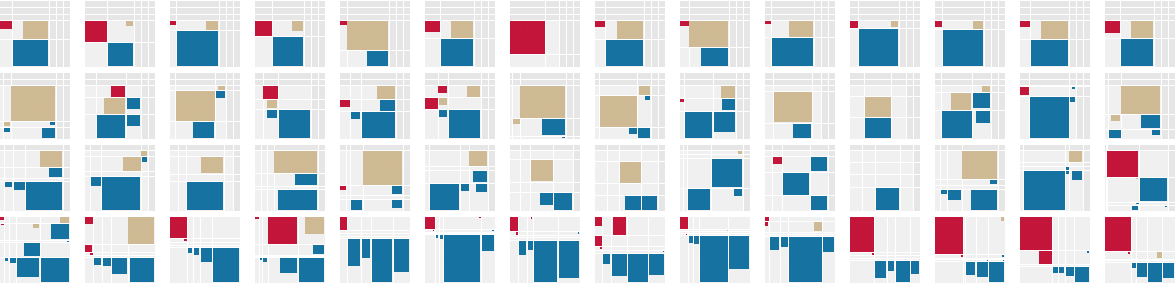
\includegraphics[width=17cm]{images/teaser.png}
%  \caption{Multivariate view with Quadmaps}
}

%% Abstract section.
\abstract{In this paper, we propose an interactive visualization called ADVISe (Annotation Dynamics Visualization) which tackles the problem of visualizing evolution in enzyme annotations across several releases of UniProt/SwissProt database. More specifically, we visualize the dynamics of the EC numbers which are a numerical and hierarchical classification scheme for enzymes, based on the chemical reactions they catalyze. An EC number consists of four numbers separated by periods and represents a progressively finer classification of the catalized reaction. The proposed interactive visualization gives a macro view of the changes and presents further details on demand such as frequencies of change types segmented by levels of generalization and specialization, as well as by enzyme families. Users can also explore entries metadata. With this tool we were able to identify trends of specialization, database growth, exceptions where EC numbers were deleted, divided or created and also changes from past annotation errors.}% end of abstract

%% ACM Computing Classification System (CCS). 
%% See <http://www.acm.org/class/1998/> for details.
%% The ``\CCScat'' command takes four arguments.

\CCScatlist{ 
Information visualization, Bioinformatics, Database dynamics, Enzymes, EC number, UniProt, SwissProt, Annotation, Processing.\\
}

%% Copyright space is enabled by default as required by guidelines.
%% It is disabled by the 'review' option or via the following command:
% \nocopyrightspace

%%%%%%%%%%%%%%%%%%%%%%%%%%%%%%%%%%%%%%%%%%%%%%%%%%%%%%%%%%%%%%%%
%%%%%%%%%%%%%%%%%%%%%% START OF THE PAPER %%%%%%%%%%%%%%%%%%%%%%
%%%%%%%%%%%%%%%%%%%%%%%%%%%%%%%%%%%%%%%%%%%%%%%%%%%%%%%%%%%%%%%%%

\begin{document}

%% The ``\maketitle'' command must be the first command after the
%% ``\begin{document}'' command. It prepares and prints the title block.

%% the only exception to this rule is the \firstsection command

\maketitle

\section{Introduction} 

In recent decades there was a significant growth of biological data generated by experimental techniques such as the new generation DNA sequencing, protein sequencing and protein structure determination. Much of these data are organized and made publicly available to the scientific community in biological databases over the Internet. According to \cite{lesk2005database} these repositories not only store biological raw data but also relevant information related to them such as literature data, protein function, relationship between a protein and its encoding gene, among other metadata.

Given that these biological databases are growing at very high rates, most of these metadata are automatically assigned. In the majority of the cases, with no laboratory experiments at all, the roles of most genes in several organisms have been reported by homology propagation \cite{brenner1999errors}. To ensure that these annotations remain reliable, studies about the confiability of the entries as well as measures of confidence should be developed. Many studies have called the attention to errors rates in the biological databases annotations \cite{devos2001intrinsic,green2005genome,jones2007estimating,schnoes2009annotation,hung2010detect}

In fact, the automatic identification of theses errors is still an open problem and several challenges have to be faced. Without laboratory experiments to verify automatically assigned annotations, it is impossible to know for certain. However, most of the studies present comparisons of diverse functional annotation methods and show they are widely incompatible what place a rough upper bound on their accuracy. 

A major step toward automatic error detection is a description of how and to what extent biological databases entries annotations evolve. In other words, we have to be capable to understand why some entries seem to be more stable and and others more volatile and what are the factors that determines this different behaviours.

The research and development of models and algorithms as well as visualization ressources are very promissing toward understanding how biological databases evolve. Interactive visualizations can be specially powerful to represent in a macro/micro perspective this voluminous, high-dimensional and complex datasets and to help users to unveil trends and exceptions in those data sets. 

\subsection{Enzyme annotations}

By the late 1950's it had become evident that the nomenclature of enzymology, in a period when the number of known enzymes was increasing rapidly, was getting out of hand. In many cases the same enzymes became known by several different names, while conversely the same name was sometimes given to different enzymes. Many of the names conveyed little or no idea of the nature of the reactions catalysed, and similar names were sometimes given to enzymes of quite different types. To meet this situation, the General Assembly of the International Union of Biochemistry (IUB) decided, in consultation with the International Union of Pure and Applied Chemistry (IUPAC), to set up an International Commission on Enzymes. Its objective was to consider the classification and nomenclature of enzymes and coenzymes, their units of activity and standard methods of assay, together with the symbols used in the description of enzyme kinetics. The Commission prepared a report,in 1961 and it was adopted and has been widely used in scientific journals, textbooks, etc. since then. The size of the Enzyme Commission number (EC number) list has increased steadily since the publication of the first report and also many corrections were done.

The  EC number is a numerical classification scheme for enzymes, based on the chemical reactions they catalyze. Every enzyme code consists of four numbers separated by periods. Those numbers represent a hierarchical progressively finer classification of the catalized reaction. For example, the code: 3.4.21.4 is a:
\begin{description}
\item [3:] hydrolase, which means the enzyme breaks a chemical bond using a water molecule.
\item [3.4:] peptidase, which means the broken bond is a peptide bond, i.e., a bond between amino acids in a protein chain.
\item [3.4.21]: endopeptidase, because it breaks an intra-chain peptide bond.
\item [3.4.21.4:] trypsin, because enzyme has the specificity of cutting close the residues arginine and lisine.
\end{description}

When a new enzyme is annotated, one can add from one to four levels of the EC number, depending on the detail of existing knowledge. In the better case, we know all about the catalyzed reaction as well as the specific substrates and products involved. However, in many cases all we know is that the molecule is an enzyme. In this case, the annotation is left "-.-.-.-". An EC number "3.4.21.-", for instance, means we don't know enzyme substrates specifically although we have information about the reaction catalyzed.

\section{Problem modeling}
\label{sec:modelling}

Based on the numerical and hierarchical natures of the Enzyme Classification number, we proposed a model to characterize the EC changes observed over several versions of UniProt/SwissProt. First of all, our focus was on visualizing what types of changes happen and with what frequency they occur. Furthermore, it is important to know the hierarchical level in which a change occurs, since an alteration in higher levels (leftmost) are more severe than in lower ones. This way, we decided to segment changes by its common prefix length together with the number of generalizations and specializations a specific EC number has suffered.

An example of an EC number change characterized by our model is shown below.

$$3.1.3.2 \rightarrow 3.1.3.5$$

The changed exemplified happened in 77 Hydrolases of release 5 to 6. Observe that the common prefix length is 3 (the first three levels from left to right remained the same), there was 1 generalization (number 2 was deleted) and 1 specialization (number 5 was written). This change means that an acid Phosphatase is now classified as a 5'-Nucleotidase.

More examples of EC moves characterized by our prefix / generalization / specialization model are provided in Table \ref{tab_ec_change}.

\begin{table*}[h]
  \caption{Example of EC numbers across consecutive database releases and our prefix / generalization / specialization model}
  \label{tab_ec_change}
  \scriptsize
  \begin{center}
    \begin{tabular}{ccccccc}
Previous & Actual & UniProt & releases & Common & Number of  & Number of \\
EC number & EC number & id & & prefix length  &  Generalizations & Specializations \\

    \hline
      -.-.-.- & -.-.-.- & Q9K5T1 & 1 to 2 & 0 & 0 & 0\\
      3.1.4.14 & 1.7.-.- & P41407 & 7 to 8 & 0 & 4 & 2 \\
      1.1.1.- & 1.-.-.- & P52895 & 5 to 6 & 1 & 2 & 0 \\
      5.3.-.- & 5.3.1.27 & P42404 & 14 to 15 & 2 & 0 & 2 \\
      2.5.1.64 & 2.5.1.- & P17109 & 13 to 14 & 3 & 1 & 0 \\
      4.1.1.22 & 4.1.1.22 & P95477 & 1 to 2 & 4 & 0 & 0 \\
    \end{tabular}
  \end{center}
\end{table*}


\section{Data set}
\label{sec:dataset}

In this work we use the biological database UniProt \cite{uniprot2012reorganizing}, which aims to provide a centralized repository of protein sequences with comprehensive coverage and a systematic approach to protein annotation, incorporating, interpreting, integrating and standardizing data from a large number of disparate sources. It is the most comprehensive catalog of protein sequence and functional annotation and has four components optimized for different uses. As stated by \cite{uniprot2012reorganizing} the UniProt Knowledgebase (UniProtKB) is an expertly curated database, a central access point for integrated protein information with cross-references to multiple sources. 
% Raquel: achei que essa parte não é muito útil no nosso contexto.
%The UniProt Archive (UniParc) is a comprehensive sequence repository, reflecting the history of all protein sequences. UniProt Reference Clusters (UniRef) merge closely related sequences based on sequence identity to speed up searches while the UniProt Metagenomic and Environmental Sequences database (UniMES) was created to respond to the expanding area of metagenomic data. 
%
%[SABRINA] ok.

In accordance with \cite{apweiler2010universal} UniProtKB consists of two sections, UniProtKB/SwissProt and UniProtKB/TrEMBL. SwissProt contains manually annotated records with information extracted from literature and curator-evaluated computational analysis. Annotation is done by biologists with specific expertise to achieve accuracy. TrEMBL contains computationally analyzed records enriched with automatic annotation and classification. As the Swiss-Prot is considered the gold standard for protein annotation, in this work we use its data to observe and analyze the changes in EC annotation.

The major releases available in the ftp of UniProt database when this study was started (March 2009) were downloaded. We analysed releases 1 (when SwissProt was integrated to UniProt) to 15 (the current release when this study was started). 

In order to check if an EC move happened we need to look at a database entry EC annotation in two consecutive releases, therefore the mentioned releases were studied in pairs and the intersection of identifiers across two consecutive releases was taken.

The total number of entries as well as the number of entries annotated with EC number and its percentage for the fifteen used releases are provided in Table \ref{tab_releases}. Table \ref{tab_pairs} shows the number of entries in the set intersection of each release pair. 


\begin{table*}[!h]
  \caption{Releases 1 to 15 of UniProt/SwissProt.}
  \label{tab_releases}
  \scriptsize
  \begin{center}
    \begin{tabular}{ccccc}
      Release & Release date & \% of & Number of & Total of entries\\
& (MM/DD/YYYY) & entries with EC & entries with EC & \\
    \hline
	1 & 12/15/2003 & 0.37 & 52,434 & 141,681 \\
	2 & 07/05/2004 & 0.38 & 57,931 & 153,871 \\ 
	3 & 10/25/2004 & 0.38 & 61,229 & 163,235 \\ 
	4 & 02/01/2005 & 0.38 & 63,221 & 168,297 \\ 
	5 & 05/10/2005 & 0.38 & 69,164 & 181,571 \\ 
	6 & 09/13/2005 & 0.38 & 74,468 & 194,317 \\ 
	7 & 02/07/2006 & 0.39 & 80,874 & 207,132 \\ 
	8 & 05/30/2006 & 0.40 & 89,245 & 222,289 \\ 
	9 & 10/31/2006 & 0.40 & 97,508 & 241,242 \\ 
	10 & 03/06/2007 & 0.40 & 105,225 & 260,175 \\ 
	11 & 05/29/2007 & 0.40 & 108,876 & 269,293 \\ 
	12 & 07/24/2007 & 0.40 & 111,230 & 276,256 \\ 
	13 & 02/26/2008 & 0.43 & 151,694 & 356,194 \\ 
	14 & 07/22/2008 & 0.43 & 168,849 & 392,667 \\ 
	15 & 03/24/2009 & 0.44 & 189,234 & 428,650 \\ 
    \end{tabular}
  \end{center}
\end{table*}


\begin{table}[!h]
  \caption{Release pairs and number of entries in the intersection. }
  \label{tab_pairs}
  \scriptsize
  \begin{center}
    \begin{tabular}{cc}
	Release & Number of \\
	pair & entries in $\cap$\\
    \hline
	1 and 2 & 141,249 \\
	2 and 3 & 151,318 \\ 
	3 and 4 & 162,812 \\
	4 and 5 & 166,933 \\
	5 and 6 & 181,005 \\
	6 and 7 & 193,382 \\
	7 and 8 & 207,069 \\
	8 and 9 & 222,181 \\
	9 and 10 & 241,189 \\
	10 and 11 & 260,065 \\
	11 and 12 & 269,152 \\
	12 and 13 & 276,011 \\
	13 and 14 & 356,036 \\
	14 and 15 & 392,597 \\
    \end{tabular}
  \end{center}
\end{table}



\section{Related work}
\label{sec:related_work}

We call attention to different contexts where information visualization techniques have been successfully used in visual analytic processes. Wikipedia articles show that evolution has motivated interesting visualization developments. In \cite{viegasetal2004}, authors investigate the dynamics of Wikipedia through an exploratory data analysis tool that was effective in revealing patterns within a given article text changes. \cite{watenbergetal2007} proposed a color scheme approach to present edit histories of Wikipedia administrators. Furthermore, many authors \cite{holt1996, lanza2001, rysselberghe2004, voineaetal2005} have studied visualizations to easy control and understand software source code evolution or to map collaborative efforts of various developers. 

In this work, we are interested in the existence and quantification of specific events of change in enzyme hierarchical annotations. As far as we are concerned, there are no other works that propose a visualization for this type of data.

\section{Technique}

The main objectives of the proposed visualization were:

\begin{enumerate}
\item to give a macro panoramic macro view of the evolution of EC number annotations
\item to allow users to explore the complete set of changes formulating and answering general questions about EC number changes
\end{enumerate}

Concerning the first objective, we would like to present at once all the changes segmented by all the possible combinations of events considering the three parameters of the model (common prefix length and number of generalizations and specializations) across all the database releases.

\subsection{Multivariate display}

We have a multivariate problem where the fundamental activity is to compare multiple instances of several variables at once and to allow users to identify similarities and differences among them. Small multiples of Tufte  \cite{tufte_envisioning} or trellis displays \cite{cleveland_trellis1,cleveland_trellis2}, as proposed by Cleveland, are a straightforward approach to present our data. They consists of splitting the data into multiple graphs that are presented at the same time in close proximity in the screen and allows to examine data in any one grahh more easily, and comparison of values and patterns among graphs with relative ease. 
According to Few \cite{few_nysi}, individual graphs display a subset of a data set divided according to a categorical variable and the several graphs differ only in terms of data. Every graph is the same type, shape, size and shares the same categorical and quantitative scales. Scales in each graph must start and end with the same values (otherwise the accurate comparison is more difficult). Graphs can be arranged horizontally or vertically or as a matrix in a meaninful order. 

Having this in mind, we proceed explaining the proposed visual representation. The basic graph of the proposed small multiple representation, which we call from now on \textit{frame}, is presented in Figure \ref{fig:technique}. It is a 2D plot where we present in x-axis the number of generalizations and in the y-axis, the number of generalizations. 
Both x and y-axes varies in the interval [0,4]. Position (0,0) from frames represents entries with no changes in the corresponding pair of versions. It is important to point out that there are prohibited positions for some lengths of common prefixes. For instance, if a change keeps a common prefix of size 3, it is impossible to have 2 generalizations. They are presented in a darked shade of gray in Figure \ref{fig:technique}.

\begin{figure}[htb]
  \centering
  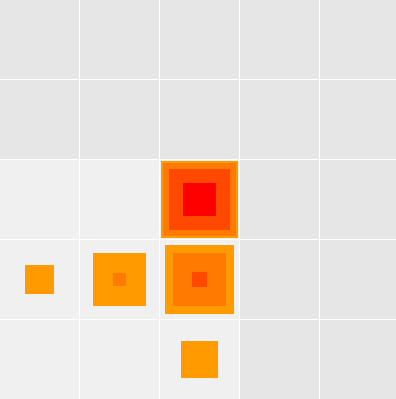
\includegraphics[width=3.5cm]{images/techniquea.png} (a) 
  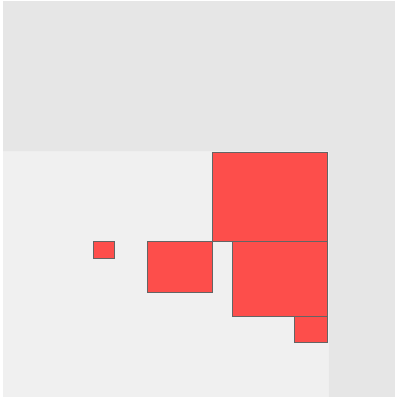
\includegraphics[width=3.53cm]{images/techniqueb.png} (b)
  \caption{Basic frames for the proposed small multiple visualization. In (a), we present the heatmap version and in (b), the squaremap. \textcolor{red}{Mudar para vers\~ao com heatmap de uma cor e com legendas}}
  \label{fig:technique}
\end{figure}

Several frames like this are then arranged in a small multiple fashion as in Figure \ref{fig:heatmap000}. In x-axis, we represent the consecutive pairs of released versions. The y-axis presents the possible common prefixes in [0,4]. 

\begin{figure*}[htb]
  \centering
  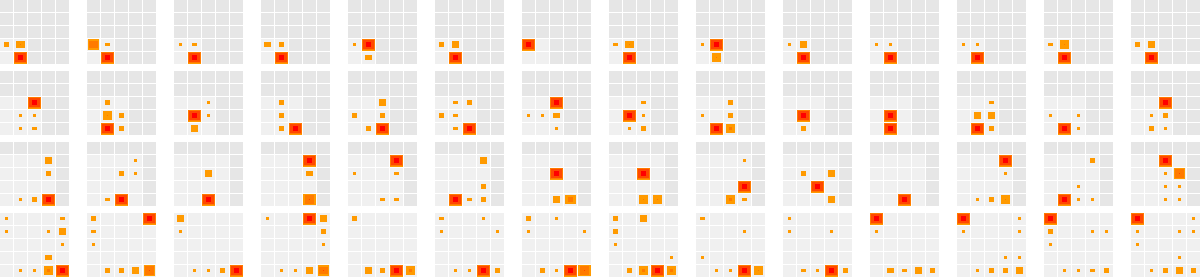
\includegraphics[width=17cm]{images/heatmap000.png}
  \caption{Multivariate view with heatmaps. \textcolor{red}{Mudar para vers\~ao com heatmap de uma cor e com legendas}}
  \label{fig:heatmap000}
\end{figure*}

\subsubsection{Heatmap}
\label{heatmap}

In a first version of the graph, we use a heatmap representation where color is a pre-attentive attribute that encodes the frequency of that configuration of change.

This representation aimed at giving an overview of the complete data evidencing trends and exceptions across the 15 releases. An interesting feature of this representation is that values in the lower right triangular matrix represents specialization and in the upper left triangular matrix, generalizations. Consequently, it is easy to recognize global trends towards generalization or specialization patterns in enzyme reaction annotations.

\subsubsection{Squaremap}
\label{squaremap}

Heatmaps present important trends in terms of generalization and specialization occurences however we see two possible drawbacks in that approach. 

Firstly, color is not a pre-attentive \textcolor{red}{???} which can preciselly encode quantitative data. For sure, one can perceive that a intense color represent a higher value than a less intense one. Hoever, it is very difficult to estimate preciselly the quantitative values from color intensities. 

The second drawback is that our heatmap presents two much blank space. According to Tufte \cite{tufte_envisioning}, the data density of a graph is the proportion of the total size of the graph that is dedicated displaying data. Tufte prefers high data density graphs as the human perceptual system is capable of detecting subtile patterns, trends and exceptions. On account of that, we decided to propose a second complementary view trying to reduce blank (non-data) space and also a representation which should use a more precise visual attribute to enconde the frequencies. 

The Squaremap representation was inspired in 2D scatterplots where the points are squares whose area represent frequency. Even though area is not the most precise visual attribute to enconde quantity, one can estimate its area through square side length which users can preciselly represent quantitative data. Notice, in Figure \ref{fig:technique}, that is easier to estimate quantities in the Squaremap (b) tnan in the Heatmap (a).

\subsection{Analytical interaction and navigation}

\subsubsection{Filtering, scales and normalization options}

The effective of the information visualization techniques hinge on the ability to clearly and accurately represent information and on the ability to interact with it to figure out what information means. Indeed, no matter how rich the display is, it will invite questions and the interaction is necessary to pursue an answer. Besides, different perspectives can lead to different insights. The proposed visualization allows pre-defined filters and different scalling and normalization options: 

\begin{enumerate}
\item log scale on the frequencies
\item normalization of frequencies by frame or globally
\item filter by only changes (removing position (0,0)) or presentation of the complete data set
\end{enumerate}

\subsubsection{Micro/macro view}

One particularly interesting way to create dense graphics is through what Tufte calls micro/macro readings \cite{tufte_envisioning}. These graphics convey one layer of information on a micro scale and another layer on a zoomed out, macro scale. One nice consequence of this technique is information is consumed hierarchically. The viewer may glance from a distance to observe an aggregate trend, and later peer in closely to examine individual pieces of that trend. Our multivariate view is a macro view of the whole changes data set. Users can click each frame and see it zoomed in a micro view. 

\subsubsection{Exploratory navigation}

Besides having a micro/macro view of the possible changes in enzyme annotation, users can click the points in the micro view and see interactive histograms of each type of change. Through these histograms users can see the enzyme families which has suffered that change. These histograms are composed by small squares representing each change and by clicking individual points users can see details about the entry. 

%\begin{figure*}[htb]
%  \centering
%  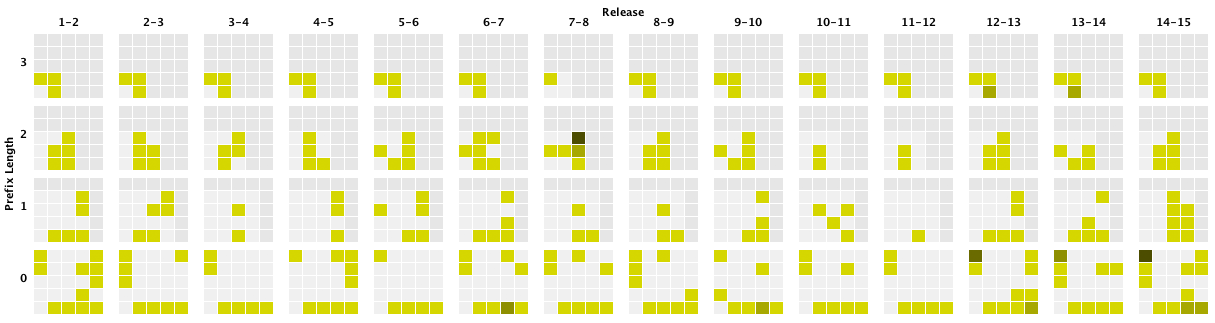
\includegraphics[width=17cm]{images/heatmap001.png}
%  \caption{Heatmap, only changes, no log scale, global normalization}
%\end{figure*}

%\begin{figure*}[htb]
%  \centering
%  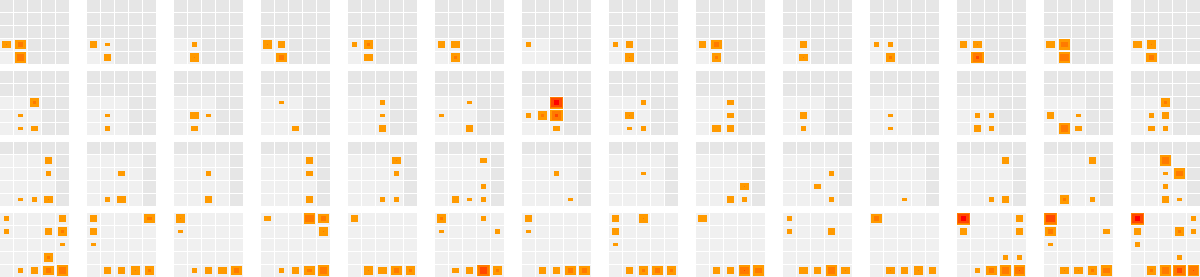
\includegraphics[width=17cm]{images/heatmap101.png}
%  \caption{Heatmap, only changes, log scale, global normalization}
%\end{figure*}

%\begin{figure*}[htb]
%  \centering
%  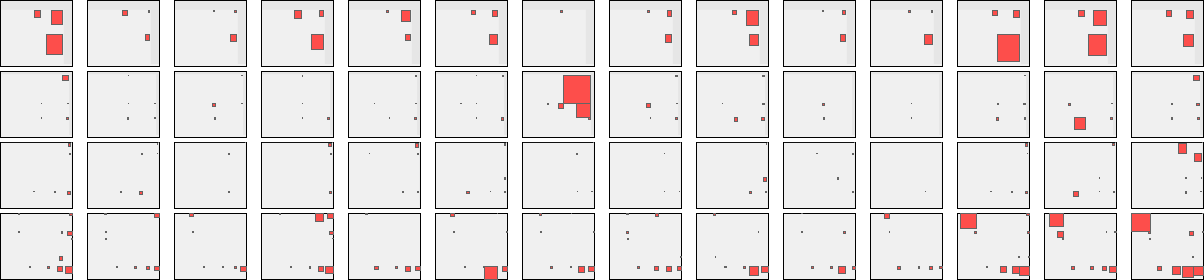
\includegraphics[width=17cm]{images/squaremap001.png}
%  \caption{Square, only changes, no log scale, global normalization}
%\end{figure*}

%\begin{figure*}[htb]
%  \centering
%  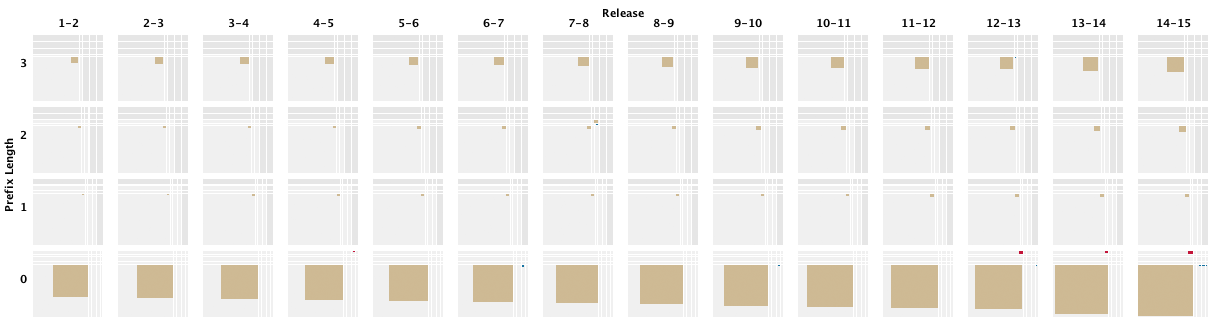
\includegraphics[width=17cm]{images/squaremap011.png}
%  \caption{Squaremap, only changes, log scale, global normalization}
%\end{figure*}

%\begin{figure}[htb]
%  \centering
%  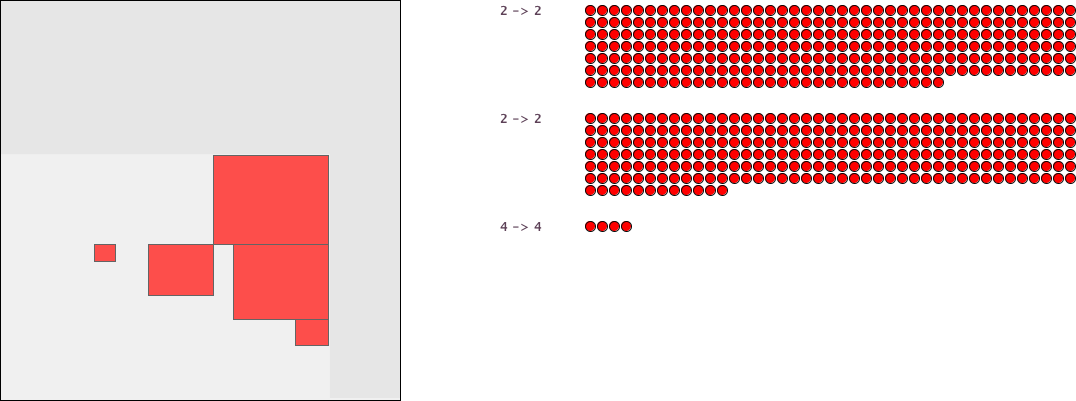
\includegraphics[width=8cm]{images/squaremap_detalhe.png}
%  \caption{}
%\end{figure}

\section{Discussions}

In this section, we describe the insights we obtained through the proposed interactive visualization.

\subsection{Trends}

\subsubsection{Stable enzyme annotations}

The most common event over the entire data set is located at the bottom left corner of each frame and it represents pairs of observed EC numbers that remained constant in a certain pair of versions. It means that the two EC numbers involved were equal (i.e. 3.1.3.2 to 3.1.3.2) or that there was no EC number (-.-.-.- to -.-.-.-).

%falar dos valores dos parametros
%falar porque isso é razoavel

\subsubsection{Generalization vs Especialization}

Consider, for each frame, a diagonal that extends from the bottom left corner to the top right corner (\textcolor{red}{marcar diagonal numa figura para dar exemplo}). The matrix of points below this diagonal, called lower right triangular matrix, represents changes in which there are more specializations than generalizations. In a similar manner, the matrix of points above this diagonal, called upper left triangular matrix, represents changes in which there are more generalizations than specializations. In the figure as a whole, the lower triangular matrices have more points than the superior ones, and therefore in the entire data set there are more specializations than generalizations.

\subsection{Exceptions} 

%Falar que nas versões 11 a 15 foram identificadas mudanças drásticas bem numerosas (deleções de 4 níveis). Colocar quantas entradas sofreram tais mudanças. Colocar exemplos biológicos do que isso significa (de acordo com a resposta do UniProt).

\subsubsection{Annotation deletion}

The four points, in the red rectangle of the last line of frames, whose parameters are $prefix = 0$, $generalization = 4$ and $specialization = 0$, represent a drastic change in which the four levels of involved EC numbers were deleted. The Table \ref{four_deletion} shows the frequencies related to each point.

\begin{table}[!h]
  \caption{Frequency of four-level EC number deletion from releases 11 to 15}
  \label{four_deletion}
  \scriptsize
  \begin{center}
    \begin{tabular}{cccc}
      Pair of releases & Frequencies\\
    \hline
      11 to 12 & 146\\
      12 to 13 &  1,357\\
      13 to 14 & 1,006\\
      14 to 15 & 1,976
    \end{tabular}
  \end{center}
\end{table}

In  UniProtKB/Swiss-Prot they try only to assign EC numbers to catalytic subunits. This means that in large protein complexes only one or a few of the subunits will be annotated with an EC number. When they discover cases where non-catalytic subunits are annotated with an EC number, they remove it completely since the subunits in question do not have any enzymatic activity on its own. Here we present three examples of UniProt/Swiss-Prot entries that experienced four-level EC number deletion from version 12 to 13. 

\begin{itemize}
\item Identifier Q6FSJ2, which was annotated as 1.10.2.2 in version 12, is subunit 7 of cytochrome b-c1, but not the subunit with reductase activity
\item Identifier Q8LX28, whose annotation was 3.6.3.14 in version 12, is subunit 8 of ATP synthase, which is part of the membrane proton channel
\item Identifier Q6AY96, which was annotated as 2.7.11.1 in version 12, is a subunit of a transcription factorm, but not the subunit with serine/threonine kinase activity.
\end{itemize}

\subsubsection{Deleted EC numbers}

In the highlighted point with parameters $prefix = 2$, $generalization = 2$ and $specialization = 2$ in versions 7-8, a total of 1900 EC number changes are represented. The three most numerous changes depicted in this point are, respectively, 2.7.1.37 to 2.7.11.1 (frequency 918), 2.7.1.112 to 2.7.10.1 (frequency 215) and 2.7.1.112 to 2.7.10.2 (frequency 165). As stated by IUBMB \cite{***}, the EC number 2.7.1.37 was deleted and divided in 2005 into EC 2.7.11.1, EC 2.7.11.8, EC 2.7.11.9, EC 2.7.11.10, EC 2.7.11.11, EC 2.7.11.12, EC 2.7.11.13, EC 2.7.11.21, EC 2.7.11.22, EC 2.7.11.24, EC 2.7.11.25, EC 2.7.11.30 and EC 2.7.12.1. The same happened to the EC number 2.7.1.112, that was deleted and divided into EC 2.7.10.1 and EC 2.7.10.2. In such cases, transferase annotations, more specifically EC 2.7.*.* (transferring phosphorus-containing groups), underwent a revision caused by a change in the EC classification system, not by a change in enzyme function annotation.

\section{Conclusion}
\label{sec:conclusion}

In this paper, we proposed a technique to visualize evolution in enzyme annotations, in special EC numbers, across several releases of UniProt/SwissProt data base. We modeled the changes of consecutive releases using parameters as the common prefix length and levels of generalization and specialization. The proposed interactive visualization gives a macro view of the changes and presents further details on demand as, for instance, frequencies of types of changes segmented by levels of generalizations and specializations as well as by the enzyme families. Users can further explore entries meta data. By visual means, we were able to evidence trends of specialization and growth of the database as well as detect several exceptions where EC numbers were deleted, divided, created or annotation errors were detected.


\acknowledgements{This work was supported by the Brazilian agencies Coordena\c{c}\~{a}o de Aperfei\c{c}oamento de Pessoal de N\'{i}vel Superior (CAPES), Conselho Nacional de Desenvolvimento Cient\'{i}fico e Tecnol\'{o}gico (CNPq), Funda\c{c}\~{a}o de Amparo \`{a} Pesquisa do Estado de Minas Gerais (FAPEMIG), Financiadora de Estudos e Projetos (FINEP) and Pr\'o-Reitoria de Pesquisa da Universidade Federal de Minas Gerais.}


\bibliographystyle{abbrv}
%%use following if all content of bibtex file should be shown
%\nocite{*}
\bibliography{2012_biovis}

%
\begin{figure*}[htb]
  \centering
  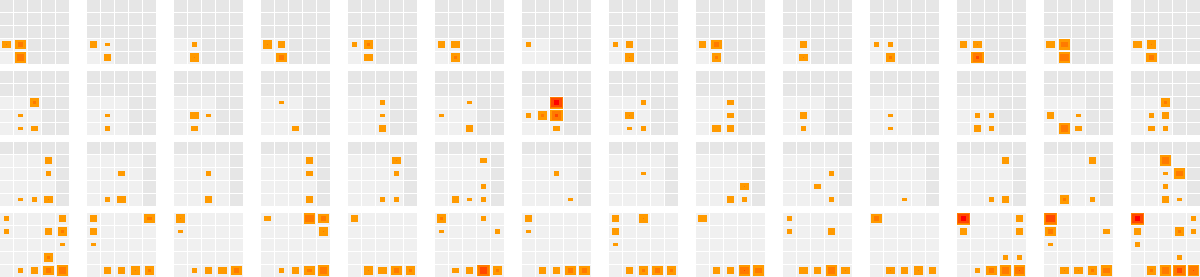
\includegraphics[width=17cm]{images/heatmap101.png} 
  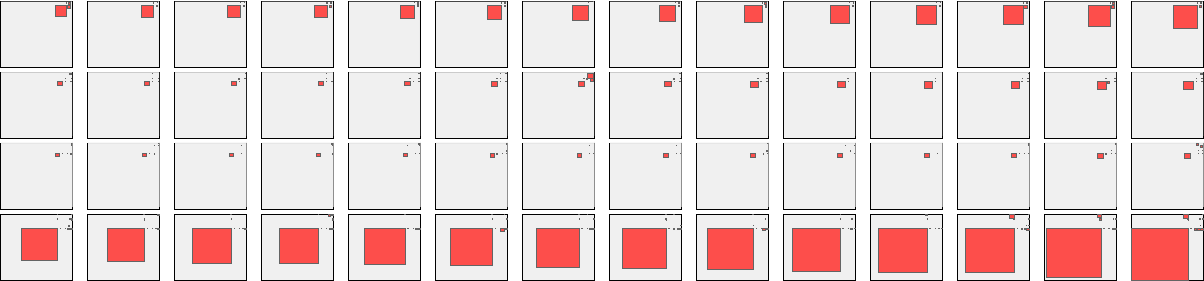
\includegraphics[width=17cm]{images/squaremap101.png}
  \caption{Log scale, Only changes, Global normalization}
\end{figure*}
\begin{figure*}[htb]
  \centering
  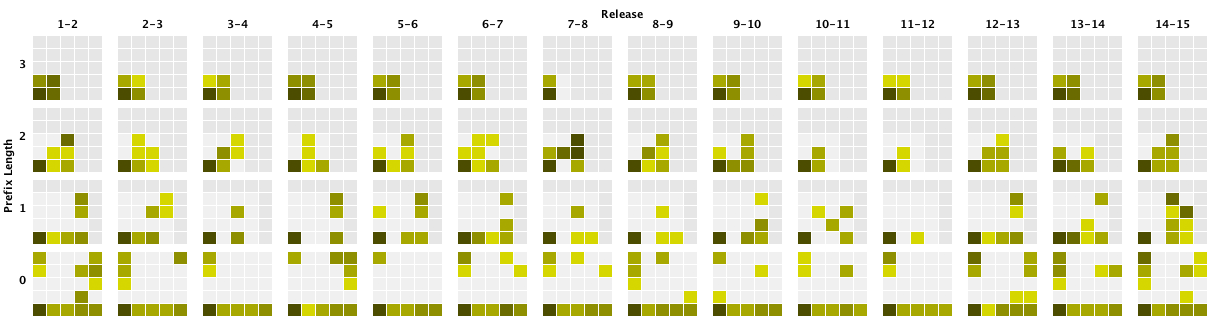
\includegraphics[width=17cm]{images/heatmap110.png} 
  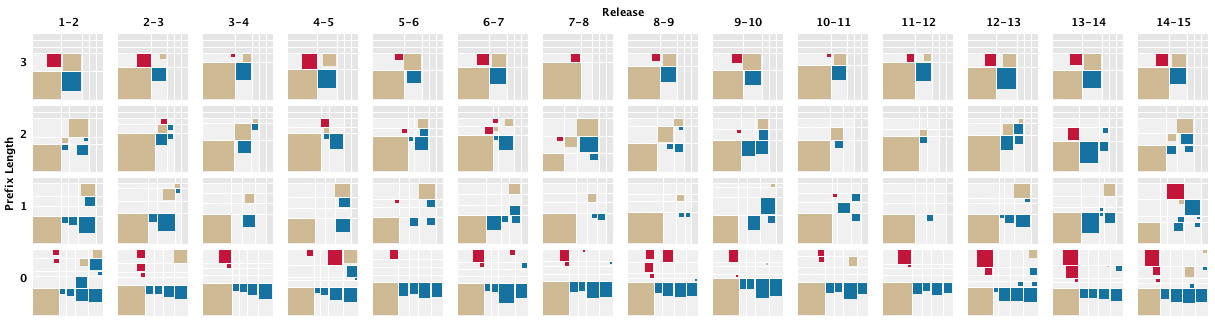
\includegraphics[width=17cm]{images/squaremap110.png}
  \caption{Log scale, Stable entries + changes, Local normalization}
\end{figure*}
\begin{figure*}[htb]
  \centering
  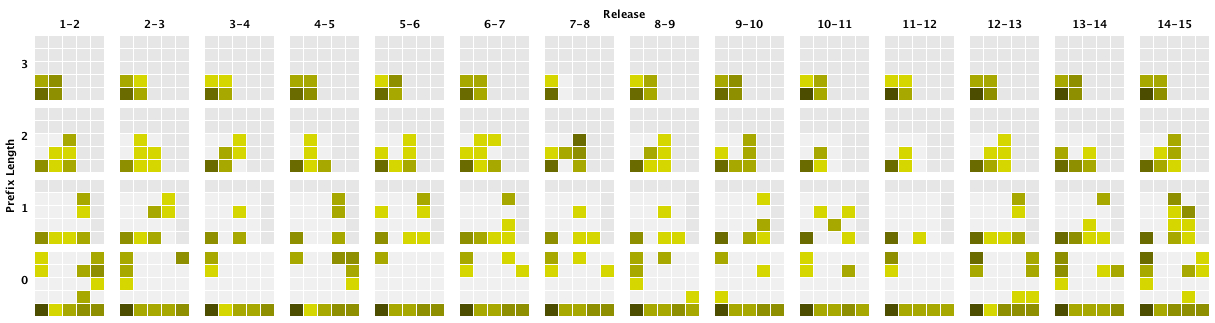
\includegraphics[width=17cm]{images/heatmap111.png} 
  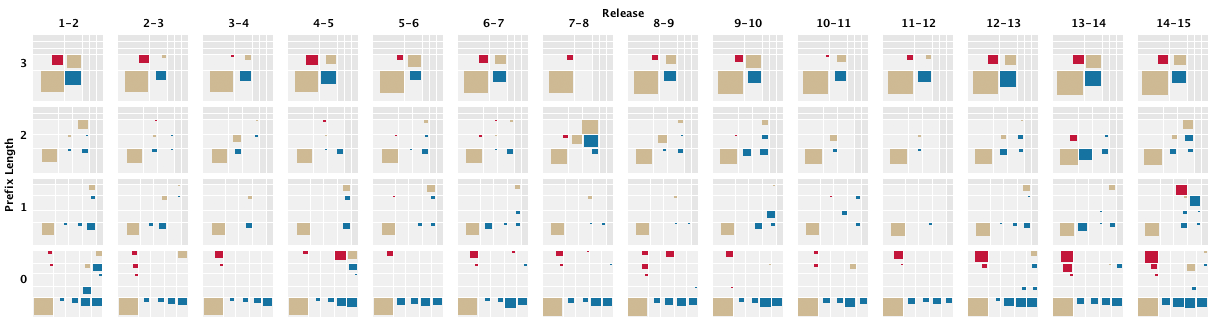
\includegraphics[width=17cm]{images/squaremap111.png}
  \caption{Log scale, Stable entries + changes, Global normalization}
\end{figure*}


\end{document}
